\chapter{Diseño e Implementación} % Main chapter title

\label{Chapter3} % Change X to a consecutive number; for referencing this chapter elsewhere, use \ref{ChapterX}
\definecolor{mygreen}{rgb}{0,0.6,0}
\definecolor{mygray}{rgb}{0.5,0.5,0.5}
\definecolor{mymauve}{rgb}{0.58,0,0.82}

\lstset{ %
  backgroundcolor=\color{white},   % choose the background color; you must add \usepackage{color} or \usepackage{xcolor}
  basicstyle=\footnotesize,        % the size of the fonts that are used for the code
  breakatwhitespace=false,         % sets if automatic breaks should only happen at whitespace
  breaklines=true,                 % sets automatic line breaking
  captionpos=b,                    % sets the caption-position to bottom
  commentstyle=\color{mygreen},    % comment style
  deletekeywords={...},            % if you want to delete keywords from the given language
  %escapeinside={\%*}{*)},          % if you want to add LaTeX within your code
  %extendedchars=true,              % lets you use non-ASCII characters; for 8-bits encodings only, does not work with UTF-8
  %frame=single,	                   % adds a frame around the code
  keepspaces=true,                 % keeps spaces in text, useful for keeping indentation of code (possibly needs columns=flexible)
  keywordstyle=\color{blue},       % keyword style
  language=[ANSI]C,					% the language of the code
  %otherkeywords={*,...},           % if you want to add more keywords to the set
  numbers=left,                    % where to put the line-numbers; possible values are (none, left, right)
  numbersep=5pt,                   % how far the line-numbers are from the code
  numberstyle=\tiny\color{mygray}, % the style that is used for the line-numbers
  rulecolor=\color{black},         % if not set, the frame-color may be changed on line-breaks within not-black text (e.g. comments (green here))
  showspaces=false,                % show spaces everywhere adding particular underscores; it overrides 'showstringspaces'
  showstringspaces=false,          % underline spaces within strings only
  showtabs=false,                  % show tabs within strings adding particular underscores
  stepnumber=1,                    % the step between two line-numbers. If it's 1, each line will be numbered
  stringstyle=\color{mymauve},     % string literal style
  tabsize=2,	                   % sets default tabsize to 2 spaces
  title=\lstname,                   % show the filename of files included with \lstinputlisting; also try caption instead of title
  morecomment=[s]{/*}{*/}%
}

En este capítulo se abordará la descripción del software desarrollado, resaltar los problemas encontrados en el análisis de una alternativa para depuración y se justifica el presente diseño propuesto de \emph{debugging} a implementado. Se exponen los criterios que han sido tenidos en cuenta a lo largo del proceso de diseño y la implementación.

%----------------------------------------------------------------------------------------
%	SECTION 1
%----------------------------------------------------------------------------------------

\section{Diseño}
\label{sec:Diseño}

\subsection{Descripción general}
\label{subsec:Descripción general}

El sistema se compone de una computadora ejecutando la depuración de un programa escrito en lenguaje CIAABOT, y la placa EDUCIAA conectado a la computadora, por medio de una interfaz, desde donde el IDE del debugger realice la comunicación con el hardware.

(mostrar una imagen de la pc con los bloques de ciaabot debugeando y conectado a la educiaa.)

\subsection{Entorno de Programación de CIAABOT debugger}
\label{subsec:Entorno de Programación}

(Se realiza la justificación del diseño) (falta implementar)


\subsubsection{Alternativa de diseño}
\label{subsubsec:Alternativas de diseño para CIAABOT debugger}

Para diseñar el software de depuración se toma como caso de estudio la depuración de un programa en lenguaje C mediante Eclipse IDE:

\begin{itemize}
	\item \emph{Plugin de eclipse arm-none-eabi-gdb}
	\footnote{Software de configuración de eclipse para usar el depurador GNU para procesadores ARM Cortex-A/R/M.}: realiza la interpretación de comandos de	GDB-MI y muestra los resultados en la interfaz gráfica del editor de texto de C en el IDE del Eclipse.
	\item \emph{arm-none-eabi-gdb}
	\footnote{Software de debug originario de linux.}: realiza el mapeo de los símbolos de C con las instrucciones en código máquina que se ejecutan en el microcontrolador (mapea las funciones al código binario en flash), para
	luego ejecutar los comandos de parar, continuar o de uso de brakpoints.
	\item \emph{OpenOCD (Open On-Chip Debugger)}\footnote{Software de código abierto que interactúa con el puerto JTAG de un depurador de hardware.}: prevee a GDB el remote interface protocol para permitirle acceder al hardware. Traduce transacciones JTAG o SWD (mediante el puerto serie sobre USB) a comandos remote-protocol de GDB. OpenOCD utiliza scripts de configuración (archivos *.cfg) donde se describe el microcontrolador a depurar y la interfaz de hardware para acceder al mismo (en adelante \emph{"Debugger HW"}).
	\item \emph{Debugger (HW)}: en el caso de la EDU-CIAA es la placa de interfaz fisica para pasar de JTAG a USB (modo puerto serie virtual). En la EDU-CIAA
	viene incluido en la misma placa que esta el micro y usa todo el circuito de hardware para debug.
	\item \emph{Microcontrolador a debuggear}: El microcontrolador posee un periferico específico para \emph{debug} con interfaz JTAG
	\footnote{Acrónimo de Joint Test Action Group, es utilizado como mecanismo para depuración de sistemas embebidos, proveendo una puerta trasera para acceder al sistema.}, teniendo acceso para modificar la RAM, Flash (externas al microcontrolador) y los registros del Microcontrolador.
\end{itemize}

Una alternativa para la programación de un software de depuración a nivel de bloques de CIAABOT es, entonces, mantener el mapeo entre los bloques de programa de CIAABOT y su C generado y comunicarse con GDB, mediante GDB-MI como lo realiza el plugin de Eclipse.

Teniendo en cuenta la complejidad de implementar lo visto anteriormente, se propone como una alternativa factible, el de emular la funcionalidad de debugger mediante la ejecución del programa de CIAABOT en la propia PC, de manera que al momento de ejecutarse los bloques gráficos de acceso a los periféricos, se realice la comunicación con la placa mediante un protocolo, y de esta manera realizar la ejecución de comandos de lectura y escritura en los periféricos que se quiere manipular.

Debido a que existe como antecedente el proyecto firmata4CIAA se decidió utilizarlo como protocolo para acceso al Hardware.


\subsubsection{Firmata}
\label{sec:Firmata}

Firmata es un protocolo genérico para comunicarse con microcontroladores desde
el software en una computadora (o teléfono inteligente / tableta, etc.).

Este protocolo fue diseñado para la comunicación directa entre un microcontrolador y un objeto de software en una computadora host Cliente Firmata. En la figura \ref{fig:componentesFirmata} se muestra el uso de firmata con Educiaa.

Firmata4CIAA es un programa que implementa el protocolo firmata en la EDU-CIAA-NXP.

\begin{figure}[h]
	\centering
	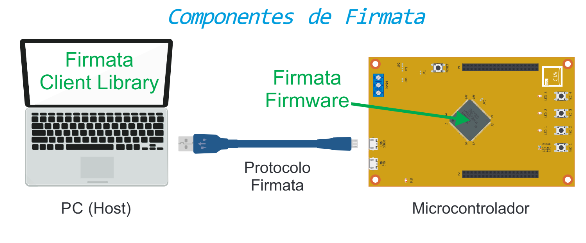
\includegraphics[scale=.80]{./Figures/componentesFirmata.png}
	\caption{Uso de firmata con la Educiaa.}
	\label{fig:componentesFirmata}
\end{figure}

\subsubsection{Johnny-Five}
\label{subsec:Johnny-Five}

Es un cliente firmata, basado en el lenguaje javaScript, de fuente
abierta. 

De esta manera se propone la comunicación entre la aplicación y la placa EDUCIAA-NXP.

\subsection{Sistema para depuración propuesto}

Después de lo visto en las secciones anteriores, se propone utilizar la siguiente secuencia de pasos:

\begin{itemize}
	\item Ejecutar un programa línea a línea, que ejecute los bloques en javascript en la PC del usuario..	
	\item Enviar comandos firmata a la placa, solo cuando se encuentre un bloque de acceso a algún periférico.
	\item Visualizar el contenido de las variables en un determinado momento de la ejecución.
	\item Instalación del protocolo firmata de la CIAA, sólo en el caso de ser necesario.
	\item Entorno gráfico amigable.
\end{itemize}

\subsubsection{Limitación}
\label{subsec:Limitación}

En este sistema propuesto, existen dos tipos de ejecución de bloques:

\begin{itemize}
	\item Bloques gráficos que acceden a los periféricos: son aquellos que usarán el protocolo firmata para enviar comandos a la placa, y mediante las funciones por UART se van comunicando con el hardware. Por ejemplo en el manejo de sensores, motores, etc.
	\item Bloques gráficos que no acceden a los periféricos: son aquellos que se ejecutan en la misma pc, por medio de javascript. Por ejemplo las sentencias loop-for, if-else, etc.
\end{itemize}

Los bloques gráficos que acceden a los periféricos, en tiempo de acceso de ejecución,
serán más lentos que si se tuviera que implentar la alternativa de diseño de
la sección \ref{sec:Alternativas de diseño para CIAABOT debugger}, ya que ese programa accedería al hardware a la velocidad en la que
se llama a las instrucciones del hardware, debido al código binario compilado
instalado en la placa.

Por el contrario, los bloques gráficos que no acceden a los periféricos, en tiempo
de ejecución, serán más rápidos, debido a que se ejecutarán directamente en la
misma PC del usuario. El programa se ejecutará dentro del contexto del VM de
javascript, que es más rápido que el código c compilado en el microcontrolador.

En conclusion si se miden los tiempos de ensayos, cuando se instala el firmware
del codigo C generado en la placa contra la ejecución de los bloques con firmata, estos tiempos no serán los mismos.

\subsubsection{Ventaja}
\label{subsec:Ventaja}

Para el usuario de CIAABOT, este método será una ventaja, ya que podrá depurar el programa sin necesidad de esperar la generación del código C a partir del programa en bloques, su compilación (especialmente en Windows) y descarga a la plataforma.


\subsection{Diseño de la Interfaz de Usuario (GUI)}
\label{subsec:Interfaz Gráfica de Usuario (GUI)}
Las funcionalidades de los botones contenidos en la barra de herramientas, explicar y mostrar los botones del debugger step in, pause, run.
funcionalidades de instalar firmata, conectar a la placa, importar proyecto....
Basicamente que hace el programa.. imagenes y texto que lo explique.

(imagenes de los botones y funcionalidades)

\subsection{Modelo computacional}
\label{subsec:Depurar un Proyecto}
explicar lo que se hace por abajo de la interfaz, las partes que intervienen, los lenguajes que usa... solo nombarlos

explicación de como se usa firmata
explicación de como se importa el mismo archivo generado en CIAABOT
explicación de generación de javascript de cada bloque
exponer las bibliotecas que se usaron



\section{Implementación}
\label{sec:Implentación}

\subsection{Descripción general}
\label{subsec:Descripción general}

\subsection{Implentación de la GUI}
\label{subsec:Implentación de la GUI}

Explicar la parte de usuario en donde se ejecuta javascript puro y johnny five.
Poner ejemplos.




\subsection{Implentación del modelo computacional}
\label{subsec:Implentación del modelo computacional}

lenguajes que se usaron, las bibliotecas que use. johnny five
componentes graficos. (Todo en mas detalle de como fue implementado)


Ejemplo de firmata con mas detalle. Muestro la tabla de Tipos de mensaje.




